\documentclass{article}
\usepackage{amsmath}
\usepackage{mathtools}
\usepackage{gensymb}
\usepackage[a4paper,inner=1.5cm,outer=1.5cm,top=2cm,bottom=0.5cm]{geometry} 
\usepackage{xcolor}                    
\usepackage{tikz}                           
\usepackage{multicol}
\usepackage{pgfplots}
\usetikzlibrary{calc}
\usetikzlibrary{intersections}
\usetikzlibrary{intersections,calc,angles,quotes}
\usetikzlibrary{shapes,arrows,positioning,decorations.pathreplacing,calc}
\usetikzlibrary{calc,angles,positioning,intersections,quotes,decorations.markings}
\usepackage{tkz-euclide}
\usetikzlibrary{backgrounds}
\usetikzlibrary{calc,through}
\usetikzlibrary{angles}
\usetikzlibrary{fadings}
\usetikzlibrary{shapes.geometric}
\usetikzlibrary{shapes.symbols}
\usepackage{draftwatermark}
\usepackage{mathptmx}

\SetWatermarkText{\textcolor{black!30}{Mathema Shukur}}
\SetWatermarkFontSize{2 cm}
\usepackage[utf8]{inputenc}
\usepackage{fontspec}

\setmainfont{[Kalpurush.ttf]}
\newfontface{\en}{[Arial.ttf]} %%this is optional, if you want to use a secondary font. Any english font is supported
\newlength\Radius
\setlength\Radius{4cm}
\begin{document} 
	\Large
	\textcolor{red}{Welcome To} 
	\\
	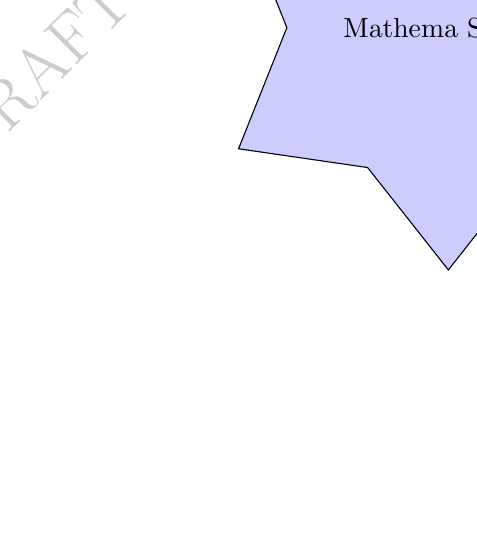
\begin{tikzpicture}
		\tikz \node [fill=blue!20,star,star points=6,draw] {Mathema Shukur };
	\end{tikzpicture}
	\\
	যাদের জন্যে প্রযোজ্যঃ  	\textcolor{magenta}{একাদশ ও দ্বাদশ শ্রেণীর শিক্ষার্থী} \\
	বিষয়ঃ \textcolor{magenta}{উচ্চতর গণিত ১ম পত্র} \\
	অধ্যায়ঃ \textcolor{magenta}{৩-সরলরেখা}\\ 
	Subtopicঃ  \textcolor{magenta}{ অন্তর্বিভক্তির সেকশন ফর্মুলা Internal Section Formula ও মধ্যবিন্দুর স্থানাঙ্ক নির্ণয় }\\
	\\
	$A(x_1,y_1)$ ও  $B(x_2,y_2)$ বিন্দুদ্বয়ের সংযোজক  সরলরেখাংশ D বিন্দুতে  $m_1:m_2$ অনুপাতে অন্তর্বিভক্ত হয়েছে।\\
	\\ 
	\begin{tikzpicture}[transform shape,scale=1]
		\draw [-latex,thick](-2,0) -- (8,0) node[right] {$x$} coordinate(x axis);
		\draw [-latex,thick](0,-2) -- (0,8) node[above] {$y$} coordinate(y axis);
		\fill[black] (0,0) circle (1.5 mm);
		\node at (-0.3,-0.3) {$\textcolor{purple}{O}$};	
		\fill[red] (2,2) circle (1 mm);
		\fill[red] (5,5) circle (1 mm);
		\fill[red] (7,7) circle (1 mm);
		\node at (5.5,6) {$\textcolor{green}{m_2}$};
		\node at (3.5,4) {$\textcolor{blue}{m_1}$};
		\node at (1.5,2.5) {$\textcolor{red}{A(x_1,y_1)}$};	
		\node at (7,7.5) {$\textcolor{red}{B(x_2,y_2)}$};
		\node at (5.8,4.7) {$\textcolor{red}{D(x,y)}$};	
			\node at (10,5) {$\textcolor{red}{x=\frac{m_1\,x_2+m_2\,x_1}{m_1+m_2}}$};			
				\node at (10,3) {$\textcolor{red}{y=\frac{m_1\,y_2+m_2\,y_1}{m_1+m_2}}$};				
		\draw[thick,blue] (2,2)--(5,5);
		\draw[thick,green] (5,5)--(7,7);
	\end{tikzpicture}
\\
 D বিন্দুর স্থানাঙ্ক $(x,y)=\left(\frac{m_1\,x_2+m_2\,x_1}{m_1+m_2},\frac{m_1\,y_2+m_2\,y_1}{m_1+m_2}\right)$\\
 \\
 	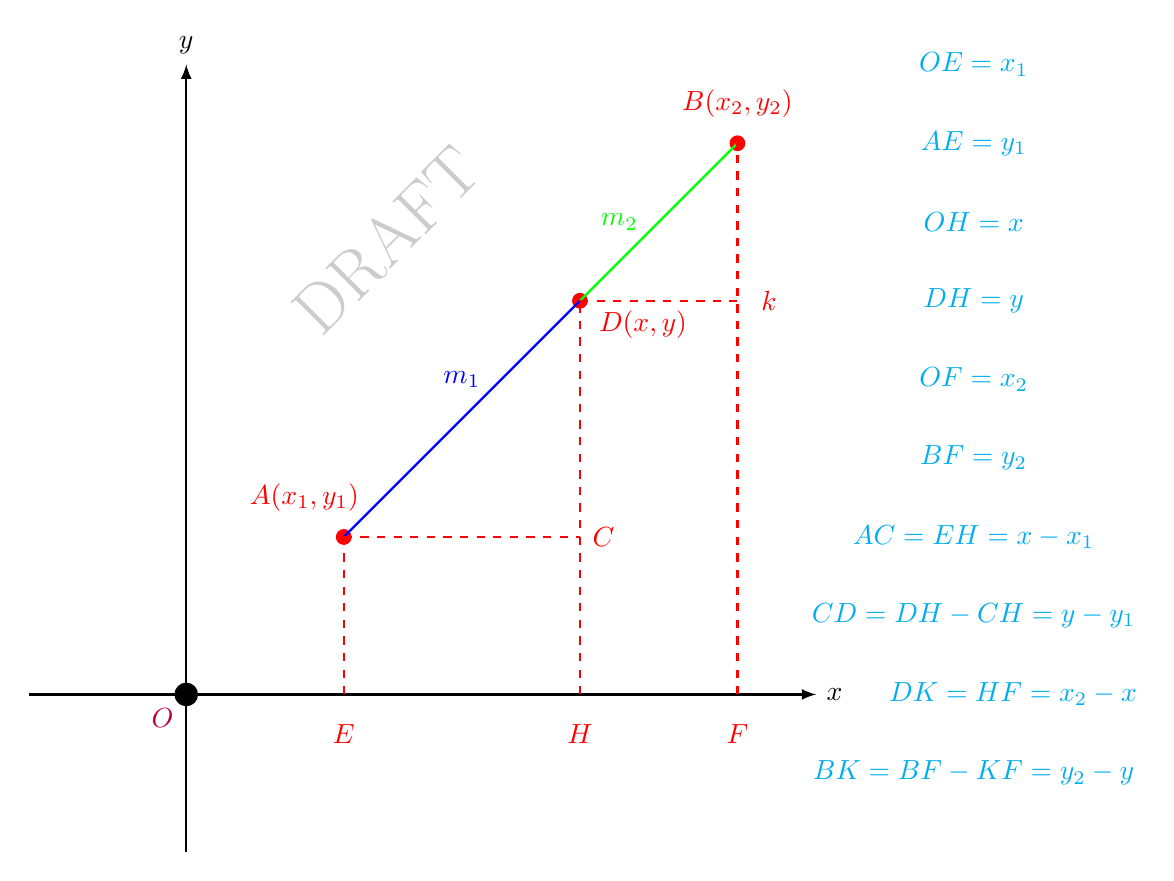
\begin{tikzpicture}[transform shape,scale=1]
 	\draw [-latex,thick](-2,0) -- (8,0) node[right] {$x$} coordinate(x axis);
 	\draw [-latex,thick](0,-2) -- (0,8) node[above] {$y$} coordinate(y axis);
 	\fill[black] (0,0) circle (1.5 mm);
 	\node at (-0.3,-0.3) {$\textcolor{purple}{O}$};	
 	\fill[red] (2,2) circle (1 mm);
 	\fill[red] (5,5) circle (1 mm);
 	\fill[red] (7,7) circle (1 mm);
 	\node at (5.5,6) {$\textcolor{green}{m_2}$};
 	\node at (3.5,4) {$\textcolor{blue}{m_1}$};
 	\node at (1.5,2.5) {$\textcolor{red}{A(x_1,y_1)}$};	
 	\node at (7,7.5) {$\textcolor{red}{B(x_2,y_2)}$};
 	\node at (5.8,4.7) {$\textcolor{red}{D(x,y)}$};	
 	\node at (2,-0.5) {$\textcolor{red}{E}$};		
 	\node at (5,-0.5) {$\textcolor{red}{H}$};	
 	\node at (7,-0.5) {$\textcolor{red}{F}$};		
 	\node at (5.3,2) {$\textcolor{red}{C}$};		
 	\node at (7.4,5) {$\textcolor{red}{k}$};					
 	\draw[thick,blue] (2,2)--(5,5);
 	\draw[thick,green] (5,5)--(7,7);
 	\draw[thick,dashed,red] (5,0)--(5,5);
 	\draw[thick,dashed,red] (2,0)--(2,2);
 	\draw[thick,dashed,red] (5,5)--(7,5);
 	\draw[thick,dashed,red] (7,0)--(7,7);
 	\draw[thick,dashed,red] (2,2)--(5,2);
 	\node at (10,8) {$\textcolor{cyan}{OE=x_1}$};		
 	\node at (10,7) {$\textcolor{cyan}{AE=y_1}$};	
 	\node at (10,6) {$\textcolor{cyan}{OH=x}$};		
 	\node at (10,5) {$\textcolor{cyan}{DH=y}$};	
 	\node at (10,4) {$\textcolor{cyan}{OF=x_2}$};		
 	\node at (10,3) {$\textcolor{cyan}{BF=y_2}$};	
 	\node at (10,2) {$\textcolor{cyan}{AC=EH=x-x_1}$};		
 	\node at (10,1) {$\textcolor{cyan}{CD=DH-CH=y-y_1}$};	
 	\node at (10.5,0) {$\textcolor{cyan}{DK=HF=x_2-x}$};		
 	\node at (10,-1) {$\textcolor{cyan}{BK=BF-KF=y_2-y}$};	
 \end{tikzpicture}
\\
এখানে ADC ও BDK ত্রিভুজদ্বয় সদৃশ (Similar)\\ 
 \begin{multicols}{2}
 	\begin{align*}
 	\frac{AC}{DK}&=	\frac{m_1}{m_2}\\
 	\\
 	\frac{x-x_1}{x_2-x}&=\frac{m_1}{m_2}\\
 	\\
 	m_1(x_2-x)&=m_2(x-x_1)\\
 	\\
 	m_1\,x_2-m_1\,x&=m_2\,x-m_2\,x_1\\
 	\\
 	m_1\,x+m_2\,x&=m_1\,x_2+m_2\,x_1\\
 	\\
 	(m_1+m_2)\,x&=m_1\,x_2+m_2\,x_1\\
 	\\
 	x&=\frac{m_1\,x_2+m_2\,x_1}{m_1+m_2}
 \end{align*}
 \\
 \begin{align*}
 	\frac{CD}{BK}&=\frac{m_1}{m_2}\\
 	\\
 	\frac{y-y_1}{y_2-y}&=\frac{m_1}{m_2}\\
 	\\
 	m_1\,(y_2-y)&=m_2(y-y_1)\\
 	\\
 	m_1\,y_2-m_1\,y&=m_2\,y-m_2\,y_1\\
 	\\
 	m_1\,y+m_2\,y&=m_1\,y_2+m_2\,y_1\\
 	\\
 	(m_1+m_2)\,y&=m_1\,y_2+m_2\,y_1\\
 	\\
 	y&=\frac{m_1\,y_2+m_2\,y_1}{m_1+m_2}
 \end{align*}
 \end{multicols}
	(1) বরিশাল বোর্ড-২০১৭\\
$(1,2)$ এবং  $(3,6)$ বিন্দুদ্বয়ের সংযোজক রেখাকে যে বিন্দু $2:3$ অনুপাতে অন্তর্বিভক্ত করে তাঁর স্থানাঙ্ক নির্ণয় কর।  \\
\\
এখানে\\ 
$m_1:m_2=2:3$,\qquad $(x_1,y_1)=(1,2)$, \qquad $(x_2,y_2)=(3,6)$\\
\begin{multicols}{2}
\begin{align*}
	x&=\frac{m_1\,x_2+m_2\,x_1}{m_1+m_2}\\
	\\
	x&=\frac{(2)(3)+(3)(1)}{2+3}\\
	\\
	x&=\frac{6+3}{5}\\
	\\
	x&=\frac{9}{5}
\end{align*}
\\
\begin{align*}
	y&=\frac{m_1\,y_2+m_2\,y_1}{m_1+m_2}
	\\
	y&=\frac{(2)(6)+(3)(2)}{2+3}\\
	\\
	y&=\frac{12+6}{5}\\
	\\
	y&=\frac{18}{5}\\
\end{align*}
\end{multicols}
সুতরাং $(1,2)$ এবং  $(3,6)$ বিন্দুদ্বয়ের সংযোজক রেখাকে $\left(\frac{9}{5},\frac{18}{5}\right)$ বিন্দু $2:3$ অনুপাতে অন্তর্বিভক্ত করে ।  \\
\\
	\begin{tikzpicture}[transform shape,scale=1]
	\draw [-latex,thick](-2,0) -- (8,0) node[right] {$x$} coordinate(x axis);
	\draw [-latex,thick](0,-2) -- (0,8) node[above] {$y$} coordinate(y axis);
	\fill[black] (0,0) circle (1.5 mm);
	\node at (-0.3,-0.3) {$\textcolor{purple}{O}$};	
	\fill[red] (1,2) circle (1 mm);
	\fill[red] (1.8,3.6) circle (1 mm);
	\fill[red] (3,6) circle (1 mm);
	\node at (2.5,4.5) {$\textcolor{green}{3}$};
	\node at (1.5,2.5) {$\textcolor{blue}{2}$};
	\node at (1,1.5) {$\textcolor{red}{A(1,2)}$};	
	\node at (3,6.3) {$\textcolor{red}{B(3,6)}$};
	\node at (3,3.6) {$\textcolor{red}{D\left(\frac{9}{5},\frac{18}{5}\right)}$};			
	\draw[thick,blue] (1,2)--(1.8,3.6);
	\draw[thick,green] (1.8,3.6)--(3,6);
\end{tikzpicture}
\\
		(2) রাজশাহী বোর্ড-২০১৯\\
	$P(4,3)$ ও $Q(-8,-5)$ বিন্দুর সংযোগ রেখাকে x-  অক্ষ যে অনুপাতে বিভক্ত করে তা বের কর।  \\
\\
ধরি,\\
	$P(4,3)$ ও $Q(-8,-5)$ বিন্দুর সংযোগ রেখাকে x-  অক্ষ $m_1:m_2$ অনুপাতে বিভক্ত করে ।  \\
	\\
$x$ অক্ষ যেকোনো রেখাকে ছেদ করলে ছেদবিন্দুর কোটি শূন্য হবে অর্থাৎ  $y=0$\\
\\
অন্তর্বিভক্তির সেকশন ফর্মুলার প্রয়োগ করে কোটি ব্যবহার করি \\
\\
\begin{align*}
	y&=\frac{m_1\,y_2+m_2\,y_1}{m_1+m_2}
	\\
	0&=\frac{m_1\,(-5)+m_2\,(3)}{m_1+m_2}
	\\
	-5\,m_1+3\,m_2&=0\\
	\\
	-5\,m_1&=-3\,m_2\\
	\\
	\frac{m_1}{m_2}&=\frac{3}{5}\\
	\\
	m_1:m_2&=3:5
\end{align*}
\begin{tikzpicture}[transform shape,scale=1]
	\draw [-latex,thick](-9,0) -- (5,0) node[right] {$x$} coordinate(x axis);
	\draw [-latex,thick](0,-9) -- (0,5) node[above] {$y$} coordinate(y axis);
	\fill[black] (0,0) circle (1.5 mm);
	\fill[red] (4,3) circle (1 mm);
	\fill[red] (-8,-5) circle (1 mm);	
		\fill[red] (-0.5,0) circle (1 mm);	
		\draw[thick,blue] (4,3)--(-0.5,0);
		\draw[thick,green] (-0.5,0)--(-8,-5);	
			\node at (2,2) {$\textcolor{blue}{3}$};
		\node at (-4.5,-3) {$\textcolor{green}{5}$};
		\node at (4,2) {$\textcolor{red}{P(4,3)}$};	
		\node at (-7,-5.5) {$\textcolor{red}{Q(-8,-5)}$};
\end{tikzpicture}
\\
	(3) কুমিল্লা বোর্ড-২০১৭\\
	$A(1,-2)$ এবং  $B(-8,1)$ বিন্দুদ্বয়ের সংযোজক রেখা BA কে  যে বিন্দু $2:1$ অনুপাতে অন্তর্বিভক্ত করে তাঁর স্থানাঙ্ক নির্ণয় কর।  \\
	\\
	এখানে\\ 
	$m_1:m_2=2:1$,\qquad $(x_1,y_1)=B(-8,1)$, \qquad $(x_2,y_2)=A(1,-2)$\\
	\begin{multicols}{2}
		\begin{align*}
			x&=\frac{m_1\,x_2+m_2\,x_1}{m_1+m_2}\\
			\\
			x&=\frac{(2)(1)+(1)(-8)}{2+1}\\
			\\
			x&=\frac{2-8}{3}\\
			\\
			x&=\frac{-6}{3}\\
			\\
			x&=-2
		\end{align*}
		\\
		\begin{align*}
			y&=\frac{m_1\,y_2+m_2\,y_1}{m_1+m_2}
			\\
			y&=\frac{(2)(-2)+(1)(1)}{2+1}\\
			\\
			y&=\frac{-4+1}{3}\\
			\\
			y&=\frac{-3}{3}\\
			\\
			y&=-1
		\end{align*}
	\end{multicols}
	সুতরাং 	$A(1,-2)$ এবং  $B(-8,1)$ বিন্দুদ্বয়ের সংযোজক রেখা BA কে  $(-2,-1)$ বিন্দুতে $2:1$ অনুপাতে অন্তর্বিভক্ত করে   \\
	\\
	\begin{tikzpicture}[transform shape,scale=1]
		\draw [-latex,thick](-9,0) -- (2,0) node[right] {$x$} coordinate(x axis);
		\draw [-latex,thick](0,-3) -- (0,3) node[above] {$y$} coordinate(y axis);
		\fill[black] (0,0) circle (1.5 mm);
		\fill[red] (1,-2) circle (1 mm);
		\fill[red] (-8,1) circle (1 mm);	
		\fill[red] (-2,-1) circle (1 mm);	
		\draw[thick,blue] (-8,1)--(-2,-1);
		\draw[thick,green] (-2,-1)--(1,-2);	
		\node at (-1.5,-0.5) {$\textcolor{red}{D(-2,-1)}$};
		\node at (-0.5,-1.8) {$\textcolor{green}{1}$};
			\node at (-6,0.7) {$\textcolor{blue}{2}$};
		\node at (-8,1.5) {$\textcolor{red}{B(-8,1)}$};	
		\node at (2.5,-2) {$\textcolor{red}{A(1,-2)}$};
	\end{tikzpicture}
\\
\vspace{5cm}
\\
\textcolor{magenta}{	$A(x_1,y_1)$ ও  $B(x_2,y_2)$ বিন্দুদ্বয়ের সংযোজক  সরলরেখাংশের মধ্যবিন্দুর স্থানাঙ্ক   $\left(\frac{x_1+x_2}{2},\frac{y_1+y_2}{2}\right)$ }\\
\\ 
কুমিল্লা বোর্ড-২০২১\\
(4) $Q(2,-2)$ এবং $R(0,4)$ এর মধ্যবিন্দুর স্থানাঙ্ক নির্ণয় কর \\
\\
 $(x_1,y_1)=(2,-2)$,\qquad $(x_2,y_2)=(0,4)$\\
 \\
  $\left(\frac{x_1+x_2}{2},\frac{y_1+y_2}{2}\right)=\left(\frac{2+0}{2},\frac{-2+4}{2}\right)=(1,1)$\\
  \\ 
  	\begin{tikzpicture}[transform shape,scale=1]
  	\draw [-latex,thick](-2,0) -- (4,0) node[right] {$x$} coordinate(x axis);
  	\draw [-latex,thick](0,-4) -- (0,6) node[above] {$y$} coordinate(y axis);
  	\fill[black] (0,0) circle (1.5 mm);
  	\fill[red] (2,-2) circle (1 mm);
  	\fill[red] (0,4) circle (1 mm);	
  	\fill[red] (1,1) circle (1 mm);	
  	\draw[thick,blue] (2,-2)--(1,1);
  	\draw[thick,green] (1,1)--(0,4);	
  	\node at (1,4) {$\textcolor{red}{R(0,4)}$};
  	\node at (2,1) {$\textcolor{red}{(1,1)}$};	
  	\node at (2.5,-2.5) {$\textcolor{red}{Q(2,-2)}$};
  \end{tikzpicture}
\end{document}